\section{Physics based interconnect reliability modelling} 
\label{sec:reliability_modeling}

Electromigration (EM) became of engineering interest since it was first observed as one of the primary failure mechanisms in aluminum IC conductors. Many researchers have studied the evolution of stress due to electromigration. Kirchheim proposed a physically based model in which generation of stress in grain boundaries during electrimigration is caused by the annihilation and generation of vacancies. Korhonen ~\cite{Korhonen:jap1993} proposed another physically based analytical model for mechanical stress evolution during electromigration in a confined metal line described by a one-dimensional equation, as follows:

\begin{equation}
\label{eq:basic_em}
\frac{\partial \sigma(x,t)}{\partial t}=\frac{\partial }{\partial x}\left[\frac{D_aB\Omega}{kT}\left(\frac{\partial \sigma(x,t)}{\partial x}+\frac{Z^*e\rho}{\Omega}j\right)\right]
\end{equation}
where $\sigma$ is the hydrostatic stress, $t$ is time, $D_a$ is the atomic diffusivity, $B$ is the effective bulk modulus, $\Omega$ is atomic volume,$k$ is the Boltzman's constant, $T$ is absolute temperature, $Z^*$ is the effective charge number, $e$ is electron charge, $\rho$ is resistivity, and $j$ is current density. Our works were mainly based on Equation
\eqref{eq:basic_em}. The advantage of this model is that the evolution of hydrostatic stress in the confined line can be calculated in a closed form, which has been widely used in EM analysis. For the sake of simplicity, we rewrote Equation \eqref{eq:basic_em} as follows:

\begin{equation}
\label{eq:basic_em_s}
\frac{\partial \sigma(x,t)}{\partial t}=\frac{\partial }{\partial x}\left[D_t\left(\frac{\partial \sigma(x,t)}{\partial x}+G\right)\right]
\end{equation}
where $D_t=\frac{D_aB\Omega}{kT}$ is the stress diffusivity affected by temperature $T$ and $G=\frac{Z^*e\rho}{\Omega}j$ is EM driving force. Moreover, $D_a=D_0e^{-\frac{E_a}{kT}}$ is the effective atomic diffusion coefficient. $D_0$ and $E_a$ stand for the pre-exponential factor and the activation energy, respectively.

\begin{figure}[!h]
\centering
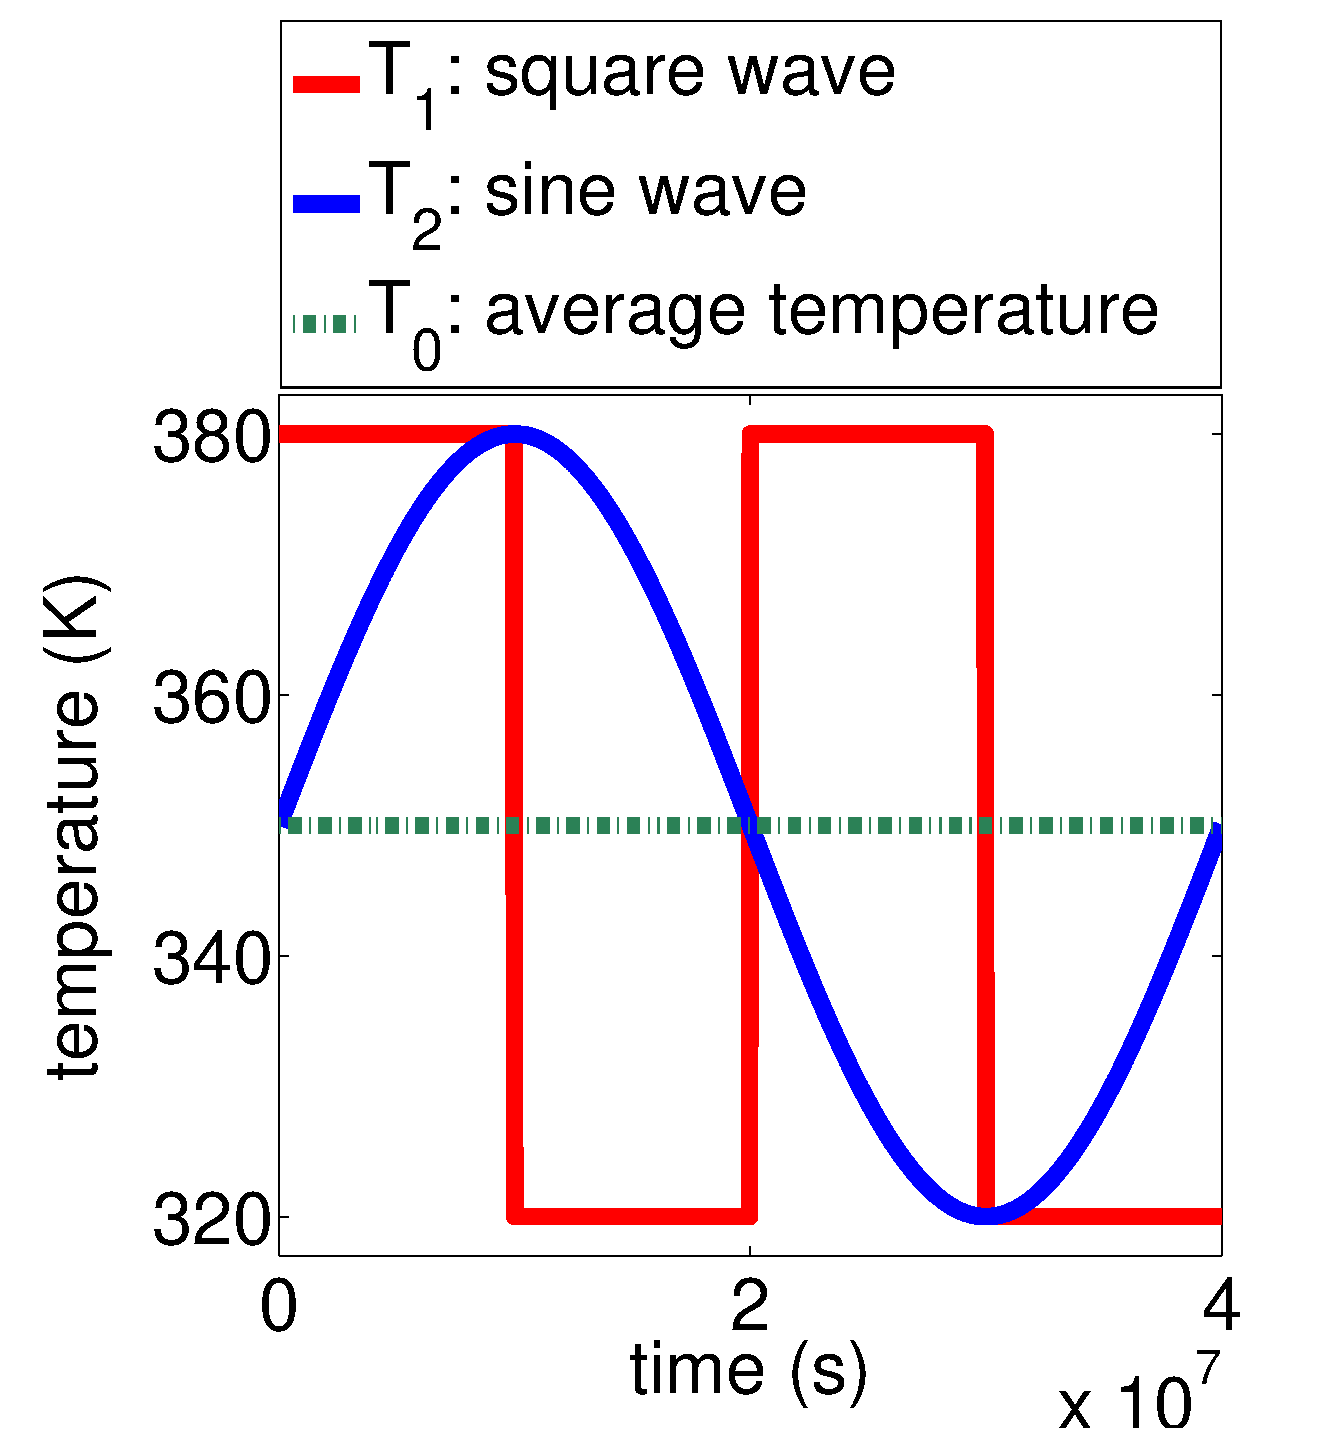
\includegraphics[width=2in]{DifferentTemperature.eps}
\caption{The different temperature function in later experiments.}
\label{fig:NTTemperature}
\end{figure}

The research for multi-branch interconnect trees is still a large and challenging problem. Due to the strong thermal-dependence of leakage power, circuit performance, IC package cost and reliability, thermal effects has become a recent major research for being a limiting factor in high performance circuit design. Among the thermal effects, varying temperature is an important part to EM analysis. We have made the EM experiments considering the changing temperature and the average temperature. In Fig.\ref{fig:NTTemperature}, we create three types of changing temperature. As we can see, function $T_0(t)$ is the average temperature of square wave temperature $T_1(t)$ and sine wave temperature $T_2(t)$. The stress evolution results for straight line interconnect tree simulated in COMSOL are showed in Fig.\ref{fig:NoteTemperature}, indicating that the relative stress variation is mostly higher than 0.5. Explicitly, we can't use average temperature to replace the changing temperature.

\begin{figure}[!h]
\centering
\subfigure[]{
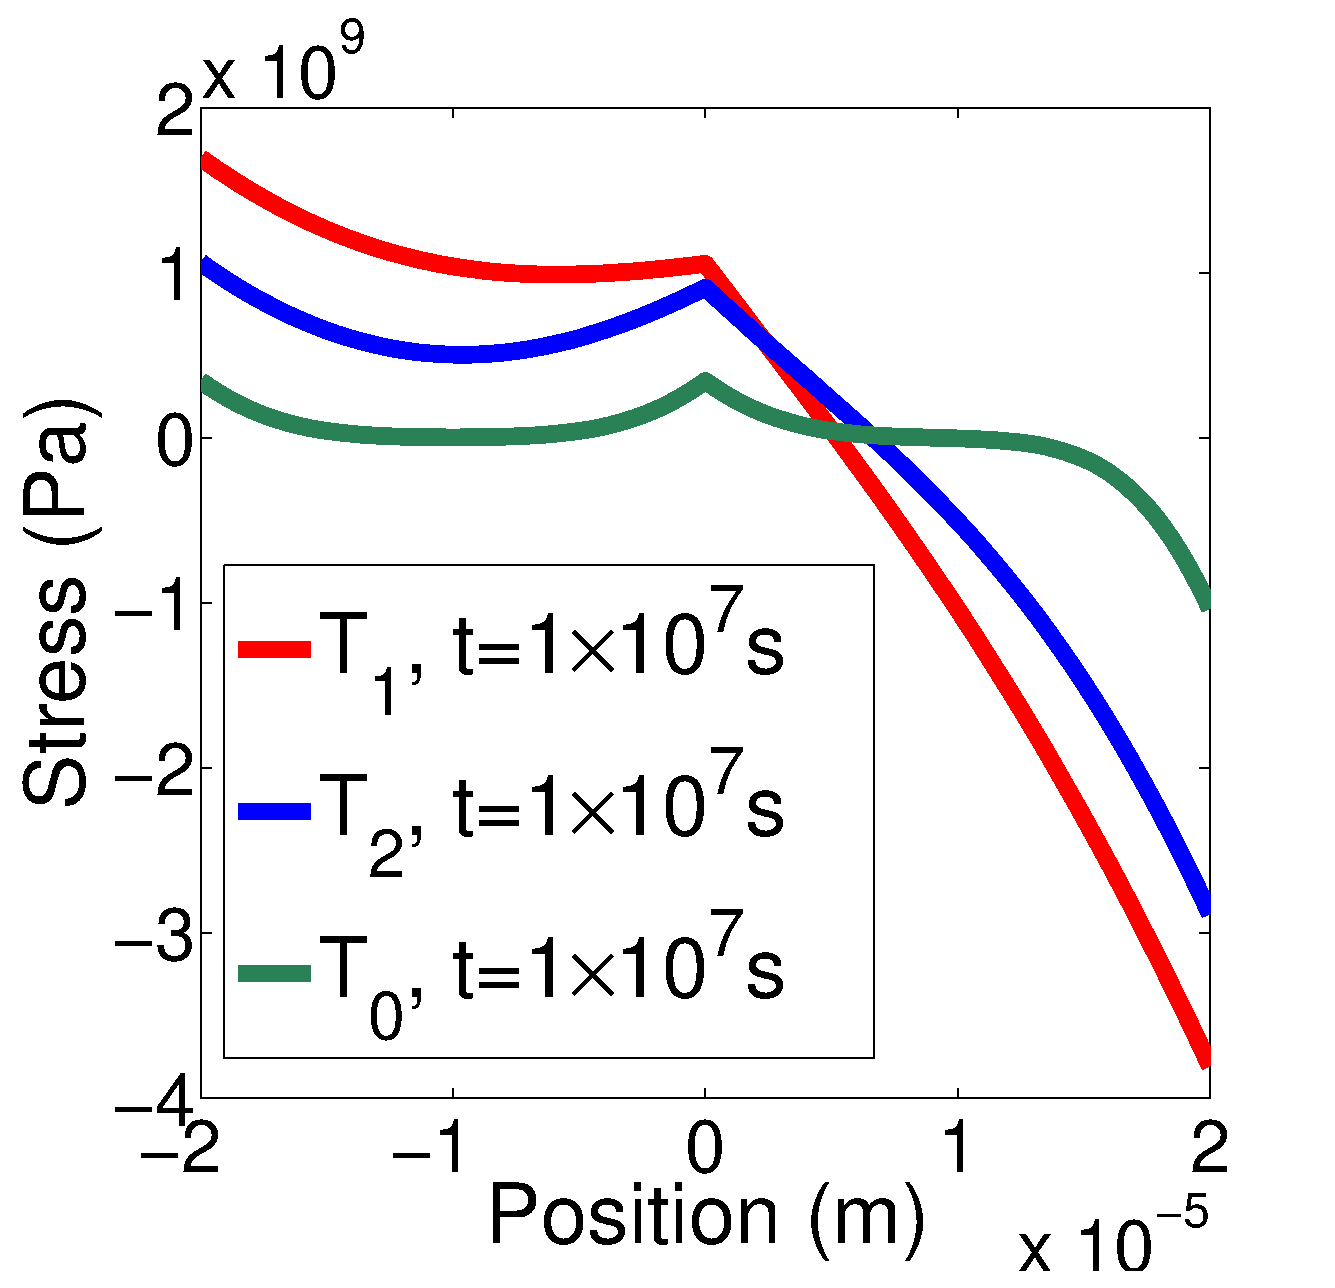
\includegraphics[width=0.45\columnwidth]{StressUnderDifferentTemperature.eps}
\label{fig:NTStress}}
\subfigure[]{
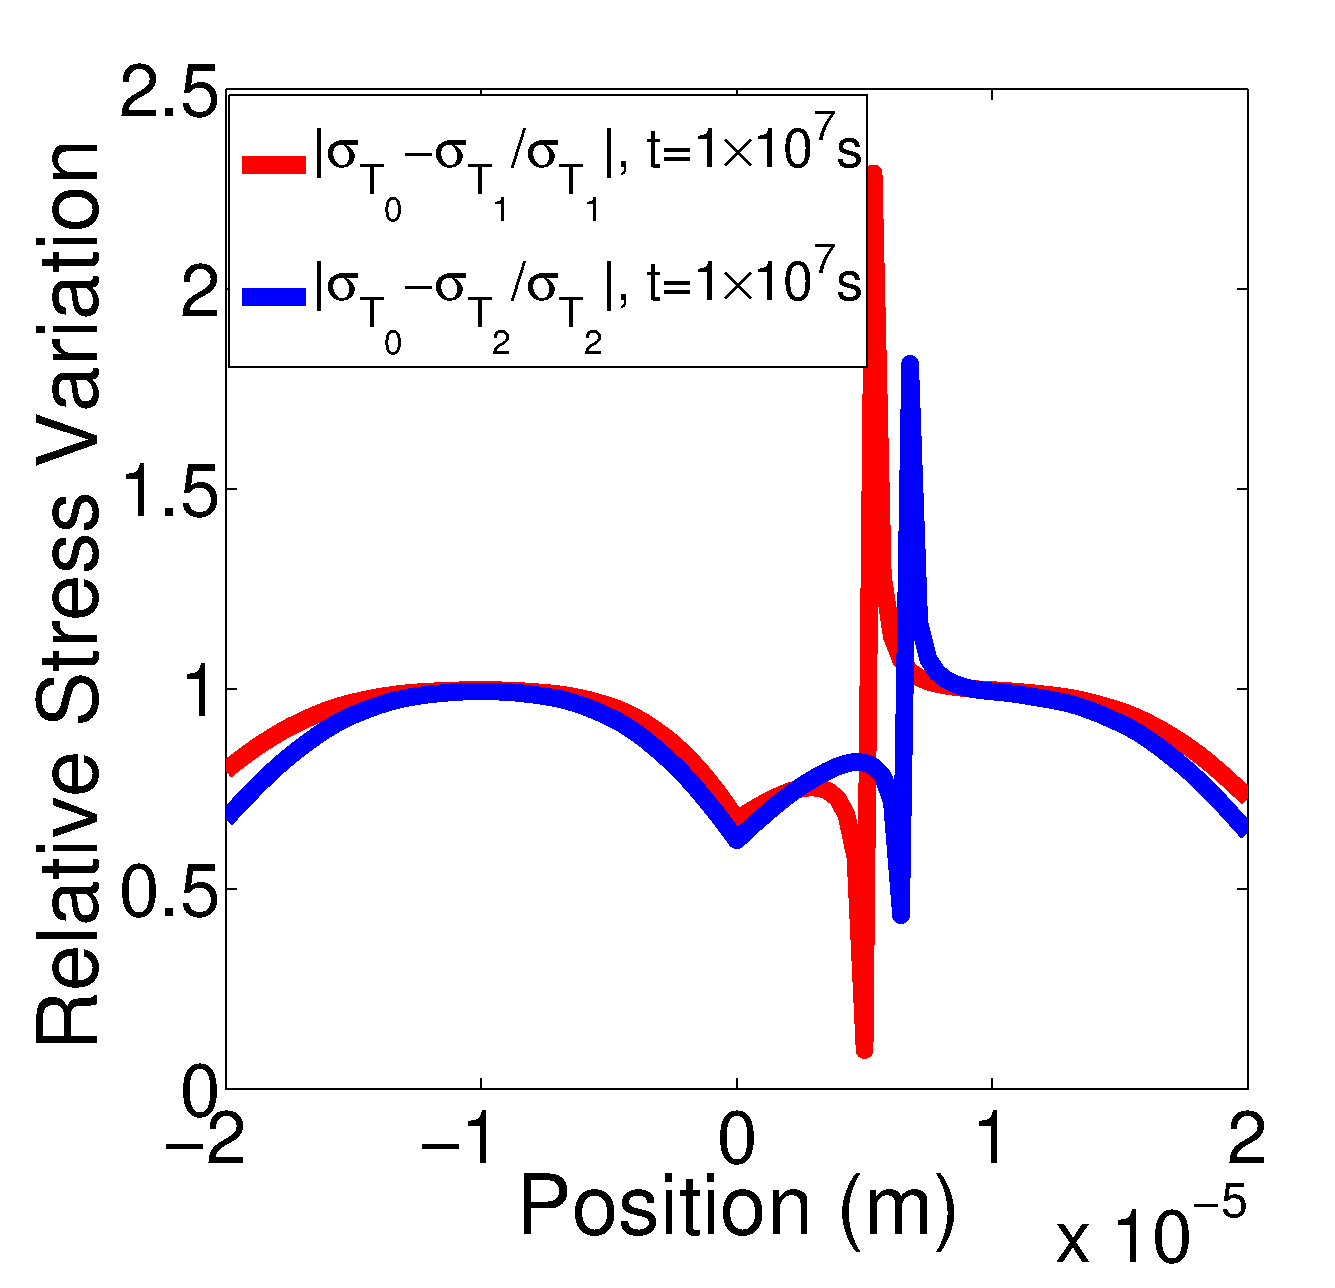
\includegraphics[width=0.45\columnwidth]{RelativeStress.eps}
\label{fig:NTRStress}}
\caption{The real results considering different temperature environment in COMSOL. (a) the stress evolution; (b) the relative stress variation.}
\label{fig:NoteTemperature}
\end{figure}

In this work, for the first time, we propose an analytic method to calculate the stress evolution considering time-varying temperature effects during the void nucleation phase for some multi-branch interconnect trees, including the straight-line there-terminal wires, the T-shaped four-terminal wires and the cross-shaped five-terminal wires. The proposed closed-form expression can be used to calculate the hydrostatic stress evolution with time-varying temperature.

The remainder of the paper is organized as follows. In Section \ref{sec:analytical_expressions}, we induce the analytical expression for the stress evolution in multi-branch interconnect tree considering constant temperature.Then we extend this model in time-varying temperature environment in Section \ref{sec:dynamic_modeling}. Experimental results for the straight-line there-terminal wires, the T-shaped four-terminal wires and the cross-shaped five-terminal wires are presented in Section \ref{sec:experimental_results}. Concluding remarks are drawn in Section \ref{sec:conclusion}.



